% Process-primary investigation map (poster pass): the dual of questions-primary.
% Spine = process (Stage 1 -> 2 -> 3); the six classes hang at each stage, colour-coded.
% Compile: pdflatex -interaction=nonstopmode
\documentclass[border=16pt]{standalone}
\usepackage{amsmath}
\usepackage{tikz}
\usetikzlibrary{positioning,fit,backgrounds,calc,arrows.meta}

\definecolor{ink}{RGB}{45,55,70}
\definecolor{cLaw}{RGB}{238,240,244}
\definecolor{cProc}{RGB}{236,238,241}
\definecolor{tProc}{RGB}{60,72,90}
\definecolor{tQ}{RGB}{96,70,150}
\definecolor{tSrc}{RGB}{42,84,140}
\definecolor{tTool}{RGB}{26,110,96}
\definecolor{tModel}{RGB}{150,104,20}
\definecolor{tFind}{RGB}{40,110,55}
\definecolor{note}{RGB}{105,105,115}

\newcommand{\sq}[1]{\textcolor{#1}{\rule{2.4mm}{2.4mm}}}
\newcommand{\rowlab}[2]{\textcolor{#1}{\textbf{#2}}\ }

\begin{document}
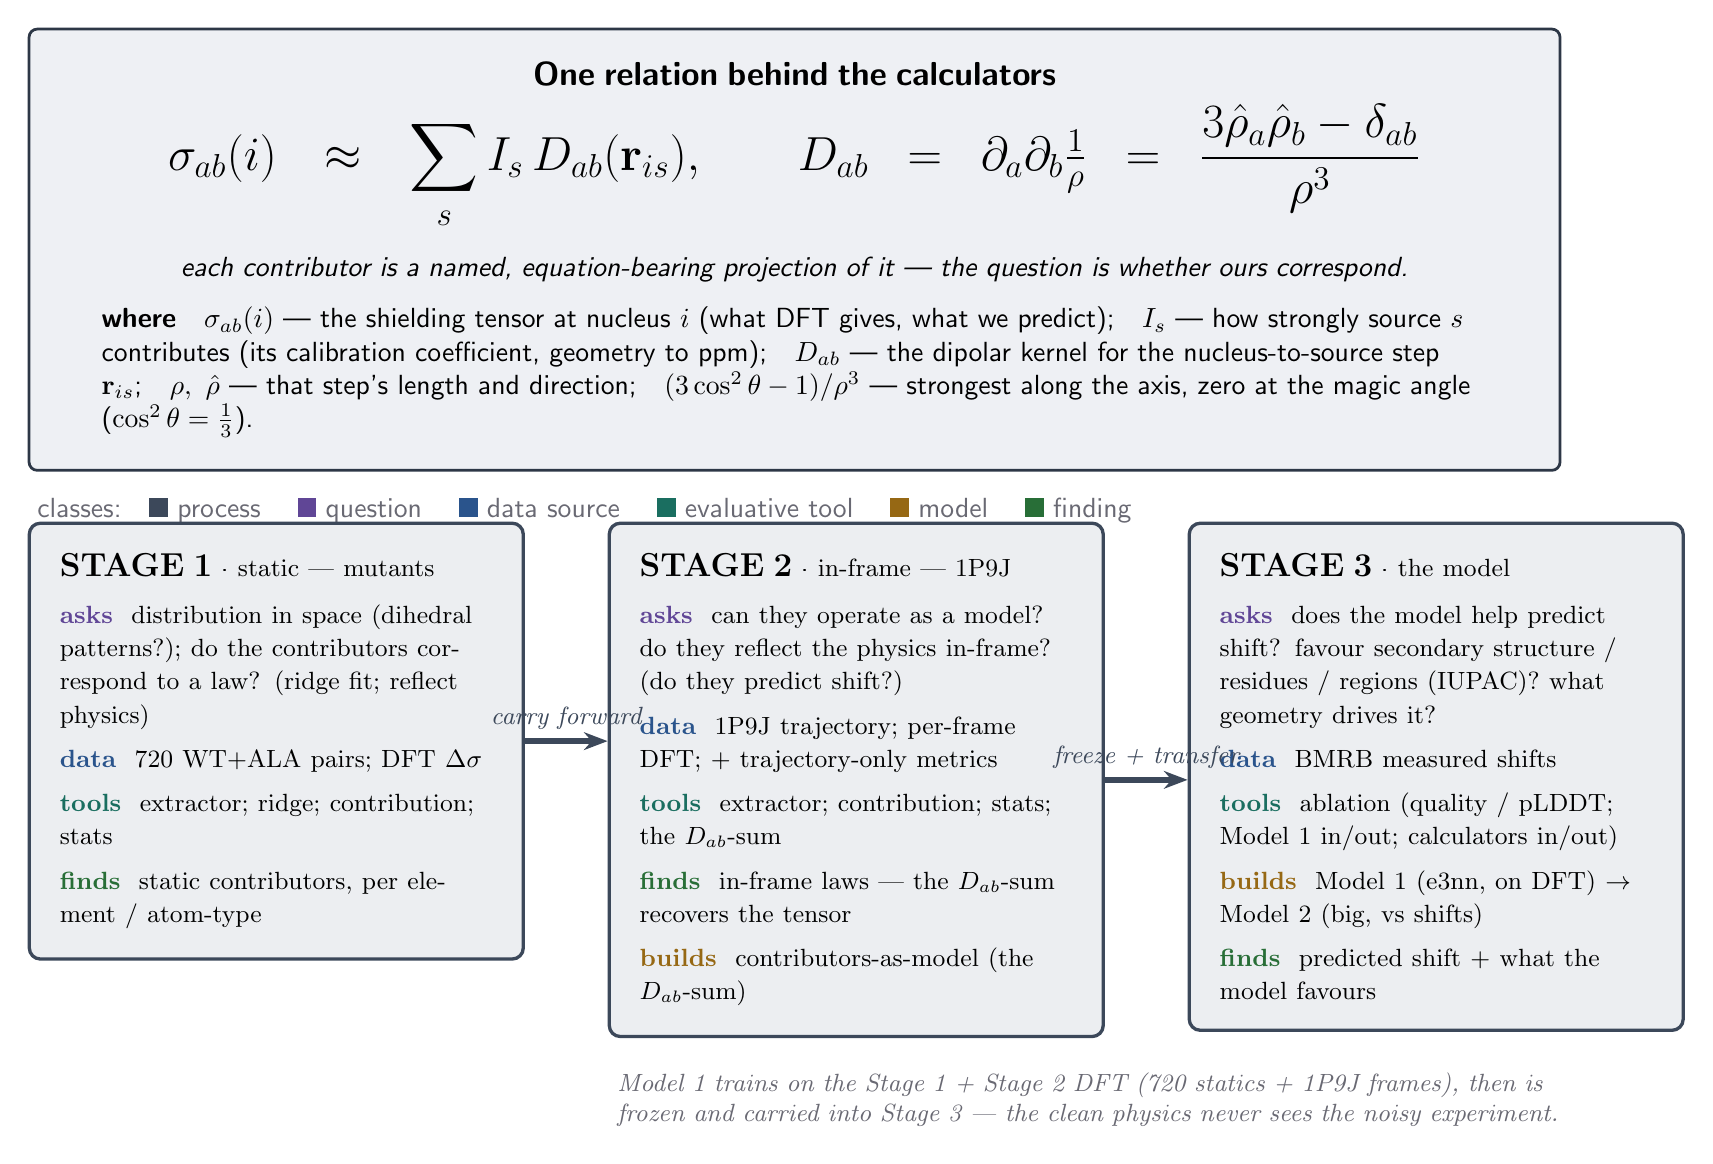
\begin{tikzpicture}[
  font=\sffamily,
  >={Stealth[length=3mm]},
  law/.style={rounded corners=3pt, draw=ink, line width=1pt, fill=cLaw, align=center, inner sep=12pt},
  stage/.style={rounded corners=4pt, draw=tProc, line width=1.2pt, fill=cProc, align=left, inner sep=11pt, text width=5.5cm, font=\normalsize},
  spine/.style={->, line width=2pt, draw=tProc},
]

% ---- the relation + grounded terms (head) ----
\node[law, text width=18.6cm] (LAW) at (0,0) {%
  {\large\bfseries One relation behind the calculators}\\[6pt]
  {\LARGE $\displaystyle \sigma_{ab}(i)\ \approx\ \sum_s I_s\, D_{ab}(\mathbf r_{is}),
   \qquad D_{ab}=\partial_a\partial_b\tfrac{1}{\rho}=\frac{3\hat\rho_a\hat\rho_b-\delta_{ab}}{\rho^{3}}$}\\[9pt]
  {\itshape each contributor is a named, equation-bearing projection of it --- the question is whether ours correspond.}\\[8pt]
  \begin{minipage}{17.6cm}\raggedright
   \textbf{where}\quad
   $\sigma_{ab}(i)$ --- the shielding tensor at nucleus $i$ (what DFT gives, what we predict);\quad
   $I_s$ --- how strongly source $s$ contributes (its calibration coefficient, geometry to ppm);\quad
   $D_{ab}$ --- the dipolar kernel for the nucleus-to-source step $\mathbf r_{is}$;\quad
   $\rho,\ \hat\rho$ --- that step's length and direction;\quad
   $(3\cos^2\theta-1)/\rho^3$ --- strongest along the axis, zero at the magic angle ($\cos^2\theta=\tfrac13$).
  \end{minipage}};

% ---- legend ----
\node[below=6pt of LAW.south west, anchor=north west, text=note] (LEG) {%
  classes:\quad \sq{tProc}~process \quad \sq{tQ}~question \quad \sq{tSrc}~data source \quad \sq{tTool}~evaluative tool \quad \sq{tModel}~model \quad \sq{tFind}~finding};

% ---- stage spine (left -> right) ----
\node[stage, below=12pt of LEG.north west, anchor=north west] (S1) {%
  {\large\bfseries STAGE 1}\ {\small\textperiodcentered\ static --- mutants}\\[5pt]
  {\small \rowlab{tQ}{asks} distribution in space (dihedral patterns?); do the contributors correspond to a law? (ridge fit; reflect physics)}\\[4pt]
  {\small \rowlab{tSrc}{data} 720 WT+ALA pairs; DFT $\Delta\sigma$}\\[4pt]
  {\small \rowlab{tTool}{tools} extractor; ridge; contribution; stats}\\[4pt]
  {\small \rowlab{tFind}{finds} static contributors, per element / atom-type}};

\node[stage, right=1.05cm of S1.north east, anchor=north west] (S2) {%
  {\large\bfseries STAGE 2}\ {\small\textperiodcentered\ in-frame --- 1P9J}\\[5pt]
  {\small \rowlab{tQ}{asks} can they operate as a model? do they reflect the physics in-frame? (do they predict shift?)}\\[4pt]
  {\small \rowlab{tSrc}{data} 1P9J trajectory; per-frame DFT; + trajectory-only metrics}\\[4pt]
  {\small \rowlab{tTool}{tools} extractor; contribution; stats; the $D_{ab}$-sum}\\[4pt]
  {\small \rowlab{tFind}{finds} in-frame laws --- the $D_{ab}$-sum recovers the tensor}\\[4pt]
  {\small \rowlab{tModel}{builds} contributors-as-model (the $D_{ab}$-sum)}};

\node[stage, right=1.05cm of S2.north east, anchor=north west] (S3) {%
  {\large\bfseries STAGE 3}\ {\small\textperiodcentered\ the model}\\[5pt]
  {\small \rowlab{tQ}{asks} does the model help predict shift? favour secondary structure / residues / regions (IUPAC)? what geometry drives it?}\\[4pt]
  {\small \rowlab{tSrc}{data} BMRB measured shifts}\\[4pt]
  {\small \rowlab{tTool}{tools} ablation (quality / pLDDT; Model 1 in/out; calculators in/out)}\\[4pt]
  {\small \rowlab{tModel}{builds} Model 1 (e3nn, on DFT) $\to$ Model 2 (big, vs shifts)}\\[4pt]
  {\small \rowlab{tFind}{finds} predicted shift + what the model favours}};

% ---- process spine arrows ----
\draw[spine] (S1.east) -- node[above, font=\small\itshape, text=tProc]{carry forward} (S1.east -| S2.west);
\draw[spine] (S2.east) -- node[above, font=\small\itshape, text=tProc]{freeze + transfer} (S2.east -| S3.west);

% ---- Model 1 note across the S1/S2 -> S3 boundary ----
\node[below=9pt of S2.south west, anchor=north west, text width=12.6cm, font=\small\itshape, text=note] {%
  Model 1 trains on the Stage 1 + Stage 2 DFT (720 statics + 1P9J frames), then is frozen and carried into Stage 3 --- the clean physics never sees the noisy experiment.};

\end{tikzpicture}
\end{document}
